This project deals with modeling and control of a refrigeration (reefer) trailer whose purpose is to maintain specific temperatures inside a box for the transportation of cargo. All sorts of products require a temperature-controlled environment which will depend and vary based on the specific product. Some examples are frozen food, dairy products, produce, medical supplies (including vaccines), and electronics. The need for transportation of perishable goods such as fresh meat, fish and fruits can hardly be questioned. This further highlights the need for high quality temperature-controlled transportation options. While reefer \textit{containers} are used in shipping, reefer \textit{trailers} are necessary when transporting to e.g. final destination facilities, warehouses, and stores.

Unlike reefer containers, reefer trailers utilize a battery as the main power supply due to the limited power delivery of the trucks they are hooked upon. Efficiency is therefore of great importance as this allows for not only greater transportation distances but also a possible reduction of the battery pack size, which is appealing because of their high cost.

The purpose of a reefer trailer is to maintain the temperature of its cargo and not actually cooling it down. It is thus expected that cargo is pre-cooled to around the desired transportation temperature before being loaded. A desired temperature is reached by cooling down air which is circulated between the cargo box and the refrigeration unit. The refrigeration unit is situated at the back of the trailer where all components besides sensors are located. Inside the refrigeration unit a refrigerant is moved between a low pressure in the evaporator and high pressure in the condenser. The evaporator extracts heat from the circulating box air and the condenser gives the heat to the ambient air outside the box. A figure of the circulation of air can be seen in \cref{fig:trailer_airflow}

\begin{figure}[h]
	\centering
	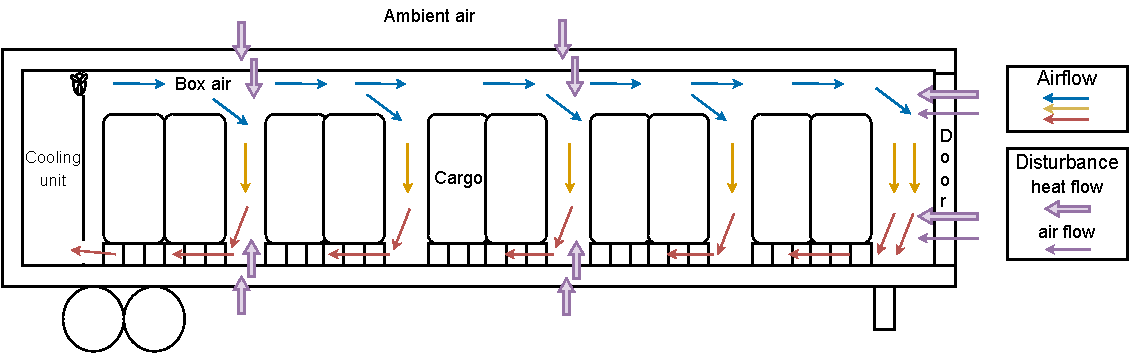
\includegraphics[width = 0.8\linewidth]{Graphics/Trailer_airflow.pdf}
	\caption{Diagram of airflow inside trailer box including disturbances}
	\label{fig:trailer_airflow}
\end{figure}

The main disturbances in the system are: 1. The air which blows in when the door is opened, 2. The continuous convection heat transfer from the outside to the inside of the box.

This project is executed in corporation with BITZER Electronics A/S as a 2nd (8th) semester project of the Masters Program in Control and Automation at Aalborg University. BITZER supplies a high fidelity model of the reefer trailer along with other relevant documentation on the system. Furthermore Kresten Sørensen from BITZER has offered counseling throughout the project.

The purpose of this project is to formulate and implement a MIMO controller for the given reefer trailer. Most control paradigms implemented in reefer systems today are still based on classical control theory such as the PID controller. The control scheme currently in place from BITZER is also made from several coupled PID controllers. BITZER wants to explore the possibility of implementing more modern control in the form of some MIMO controller, which could potentially reduce energy consumption while maintaining a proper temperature of the cargo.

The construction of a controller will require a model of the refrigeration system and as such a controller model will be made to this end. In order to evaluate the controller performance it will be benchmarked against the control scheme currently in place at BITZER.